\documentclass[10pt]{beamer}

\usetheme[progressbar=frametitle]{metropolis}
\usepackage{appendixnumberbeamer}

\usepackage{booktabs}
\usepackage[scale=2]{ccicons}

\usepackage{subfig}

\usepackage{xspace}
\newcommand{\themename}{\textbf{\textsc{metropolis}}\xspace}


\usepackage[bookmarksopen=true]{hyperref}
\usepackage{xcolor}
\usepackage{graphicx}
\usepackage[group-separator = {,}]{siunitx}


\newcommand{\faro}[0]{FARO\textsuperscript{\textregistered}\space}
\newcommand{\farons}[0]{FARO\textsuperscript{\textregistered}}

% Use metropolis theme
\title{Hyper Parameter Optimization \\using Machine Learning}
\date{July, 2021}
\author{{Nuno Costa} \\
{\textit{ISEP Advisor}: Carlos Ramos} \\
{\textit{External Advisor}: Hooshiar Zolfagharnasab}}
\institute{Polytechnic of Porto - School of Engineering (ISEP)}


\begin{document}

  \maketitle
  \section{Introduction}
  \begin{frame}{\faro Overview}
    \begin{columns}
      \begin{column}{0.6\textwidth}
        \faro is a market leader in the 3D metrology market with over US \$ 150 M of gross profit in 2020. It produces a large variety of devices (contact and non-contact measurement arms, laser scanners) and a suite of software products which integrate the devices into the customers workflow.
      \end{column}
      \begin{column}{0.5\textwidth}
        \begin{figure}
        \centering
        
\includegraphics[width=0.7\textwidth]{images/faro_logo.png}
        \caption{\faro logo}
        \end{figure}
      \end{column}
    \end{columns}
  \end{frame}
  \begin{frame}{\faro Devices}
    \begin{columns}
      \begin{column}{0.30\textwidth}
        \begin{figure}
          \centering
          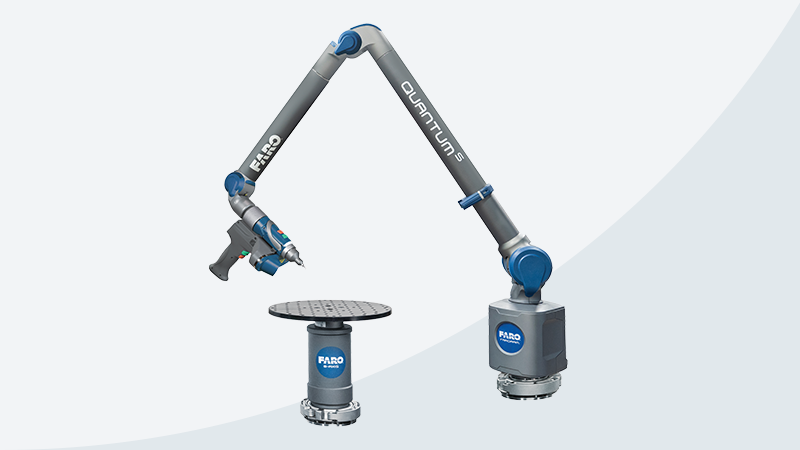
\includegraphics[width=\textwidth]{images/faro_quantum_s_arm.png}
          \caption{\newline\faro Quantum S \newline Arm}
        \end{figure}
      \end{column}
      \begin{column}{0.30\textwidth}
        \begin{figure}
          \centering
          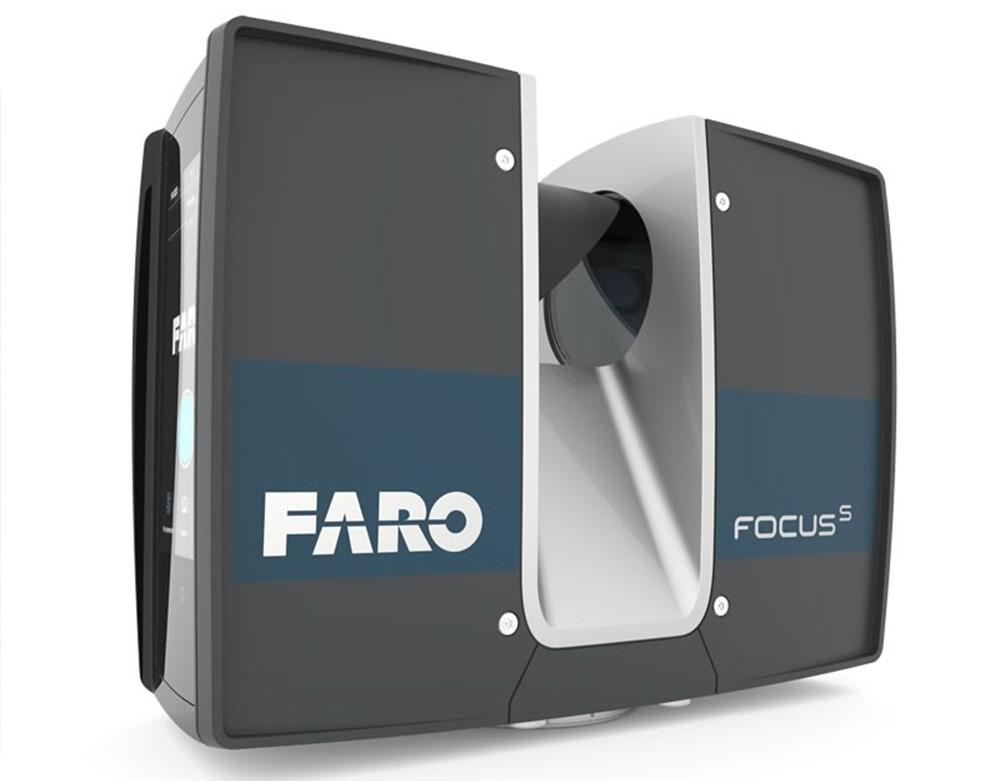
\includegraphics[width=\textwidth]{images/faro_scanner.jpg}
          \caption{\newline\faro Focus Laser Scanner}
        \end{figure}
      \end{column}
      \begin{column}{0.30\textwidth}
        \begin{figure}
          \centering
          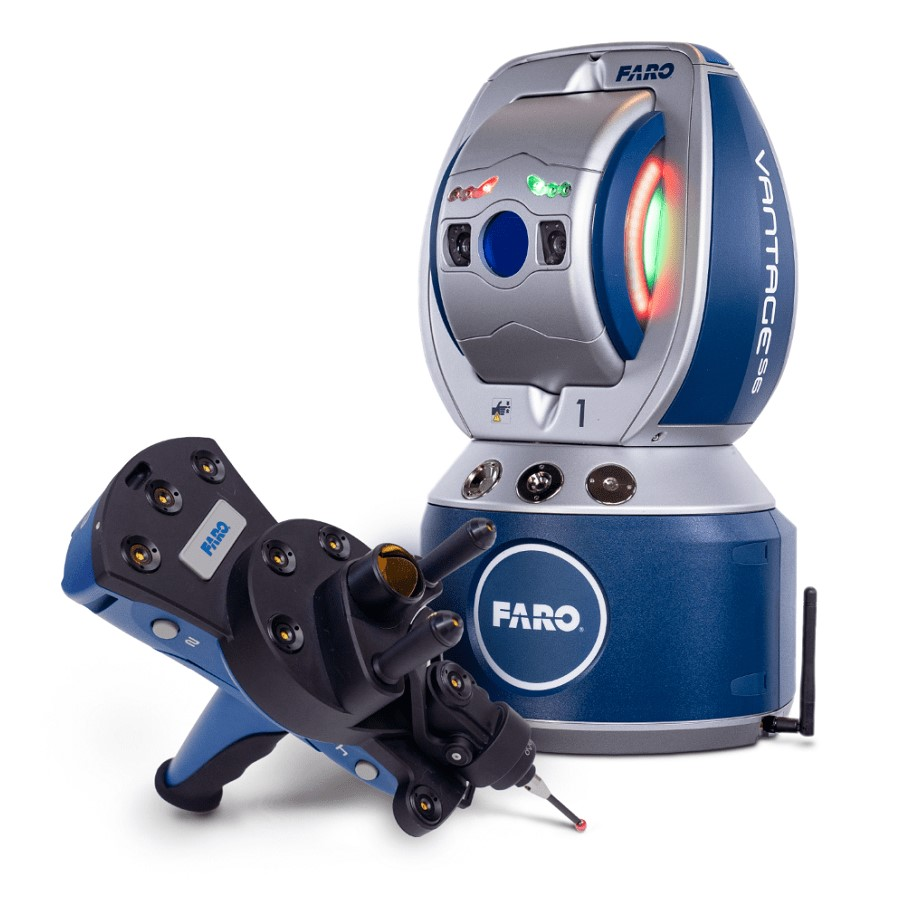
\includegraphics[width=\textwidth]{images/faro-probe.jpg}
          \caption{\newline\faro Vantage Laser Tracker}
        \end{figure}
      \end{column}
    \end{columns}
  \end{frame}
  \begin{frame}{Problem Description}
    \faro is investing heavily  in machine learning within its software suite. As such, there is a need for algorithm training tools that integrate into \faro codebase.

    This project focuses on demonstrating successful usage of these tools with \faro software, specifically a function within CAM2\textsuperscript{\textregistered}, one of \faro software offerings. 
  \end{frame}
  \begin{frame}{Objectives}
    The objective of this internship was to create a solution for hyper parameter optimization (HPO) in software solutions developed by \farons. These main goals were defined:
    \begin{itemize}
      \item Develop 3 algorithm training solutions
      \item Develop meaningful unit tests for these solutions
      \item Integrate the solutions into pre-existing software
      \item Demonstrate value by solving real world issues in CAM2\textsuperscript{\textregistered}
    \end{itemize}
  \end{frame}

  \section{State of the Art}
  \subsection{Related Works}
  \begin{frame}{Related Works}
    With regards to related works, we have explored the existing field of hyper parameter optimization. This field has a long history, dating back to the 1990s. Its contributors have produced a variety of solutions to the problem at hand. These solutions can be divided into 2 categories: black-box optimization and multi-fidelity optimization.
  \end{frame}
  \begin{frame}{Related Works}
    \begin{figure}
          \centering
          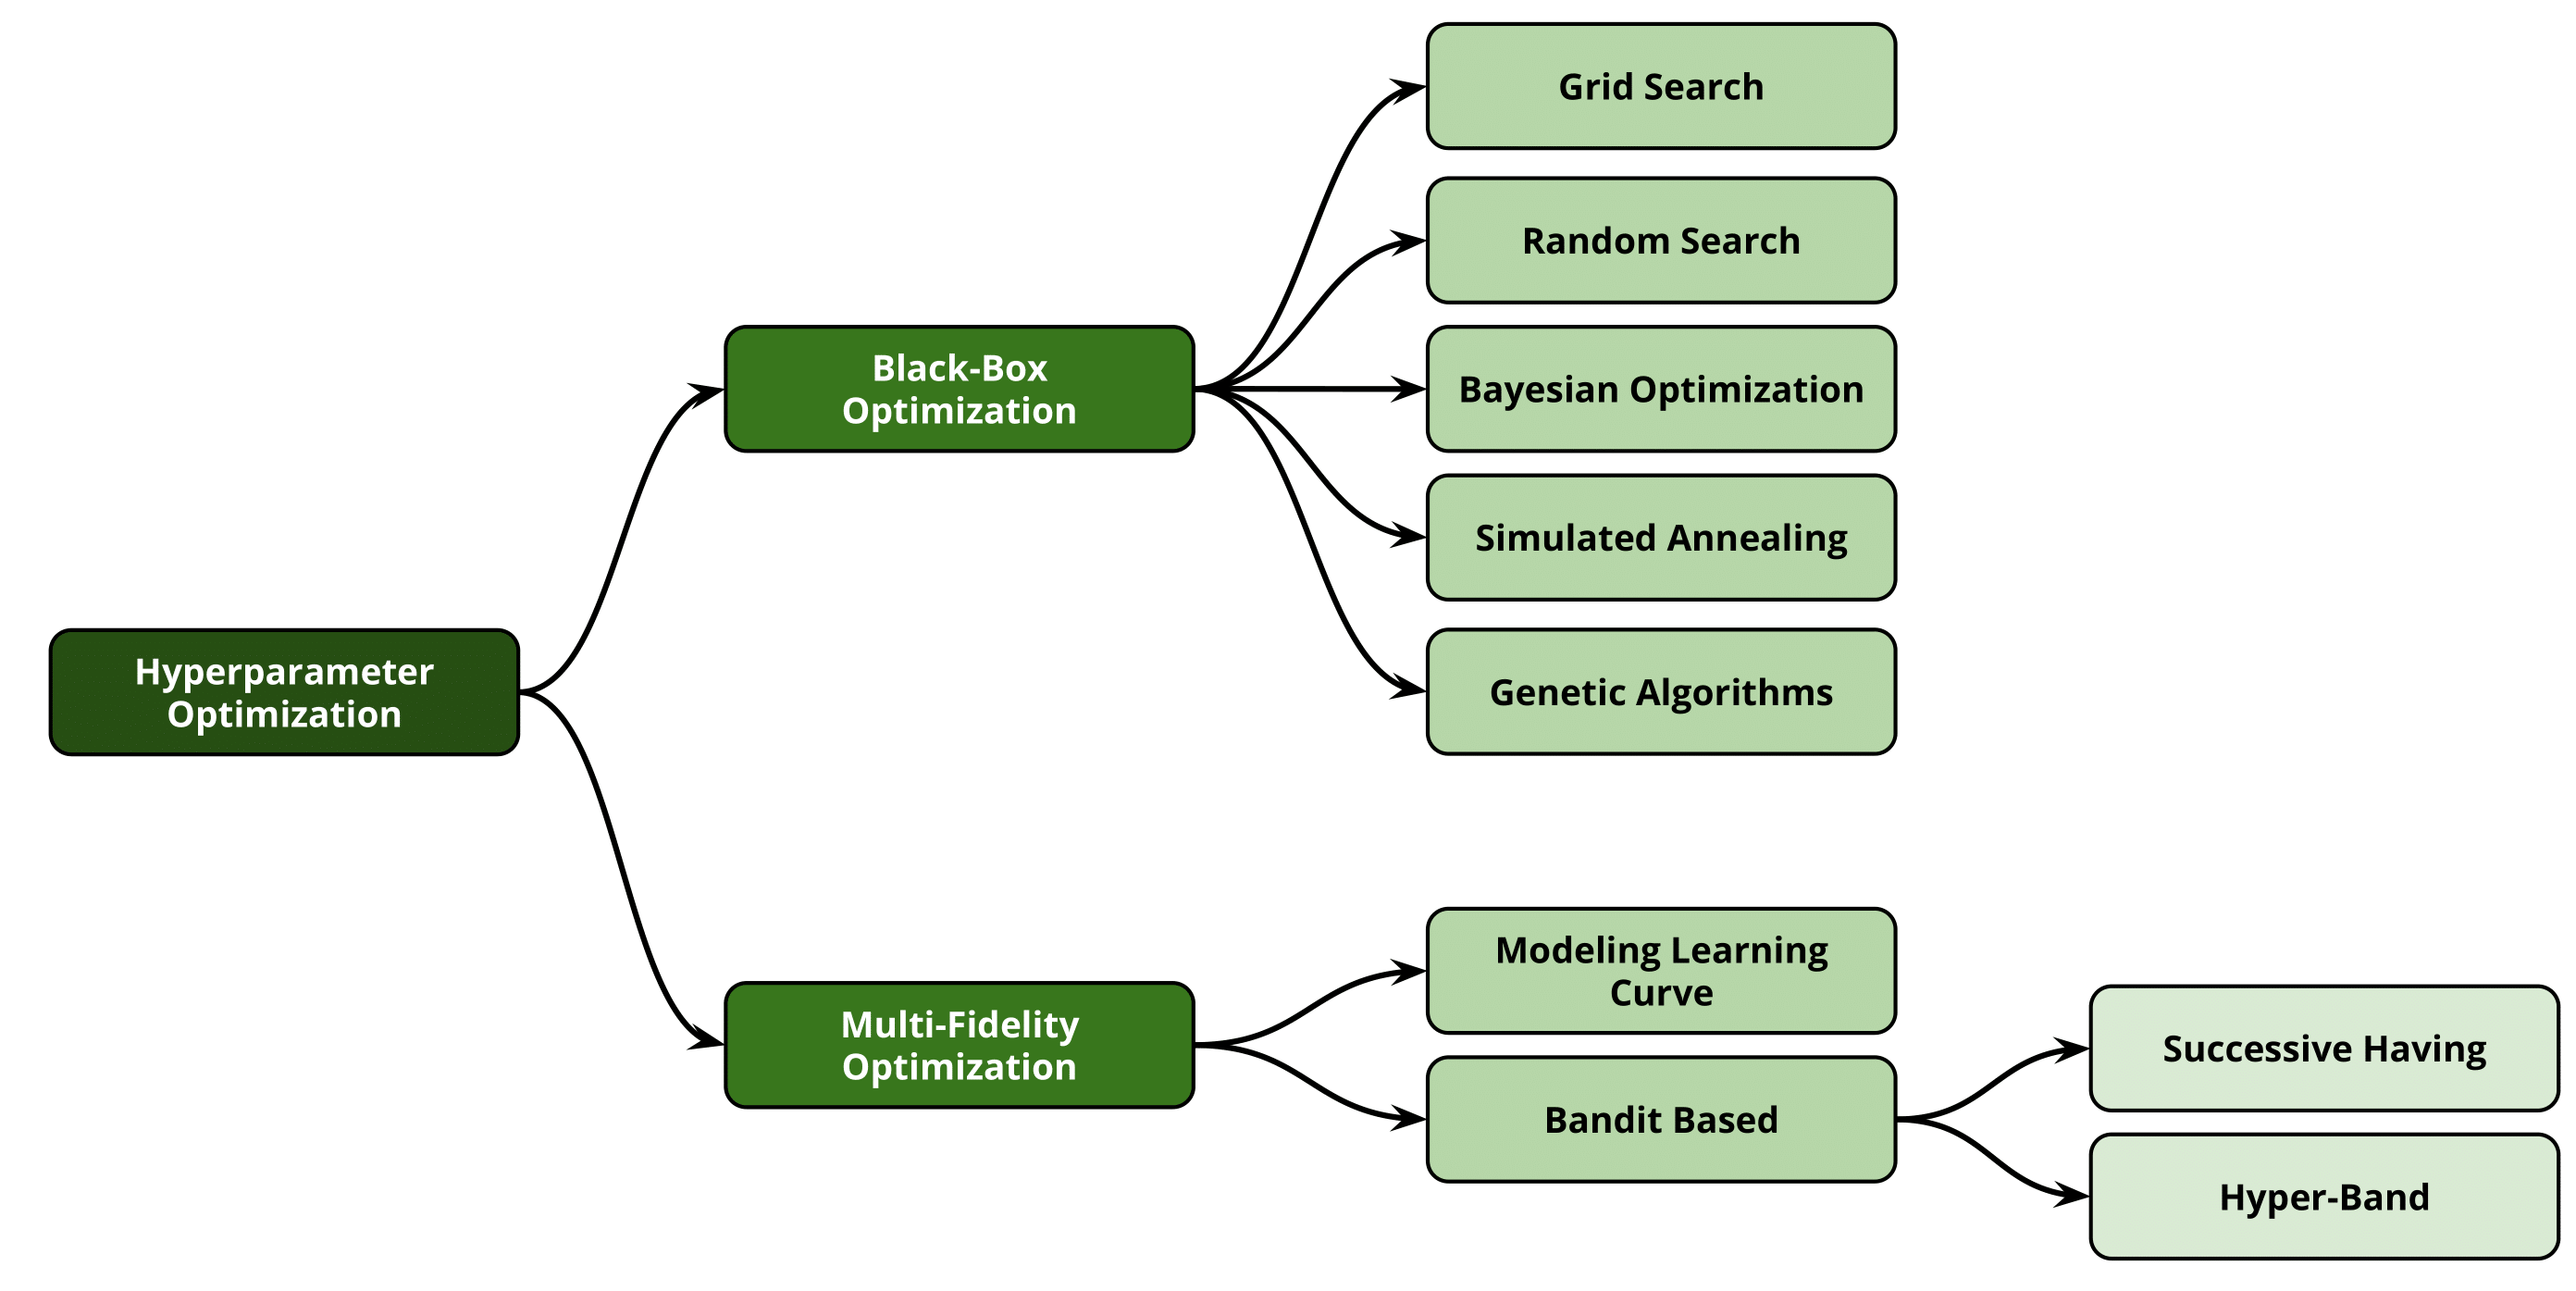
\includegraphics[width=\textwidth]{images/state_art-taxonomy_optimizers.png}
        \end{figure}
  \end{frame}
  \begin{frame}{Black-Box Optimization Algorithms}
    Black-box optimization algorithms treat the problem function as a black-box (a process that is not analytically available).
    \begin{itemize}
      \item{Grid Search}
      \item{Random Search}
      \item{Simulated Annealing}
      \item{Bayesian Optimization}
      \item{Population Based Optimization}
      \item{Genetic Algorithms}
      \item{Gradient-based Optimization}
      \item{Spectral Optimization}
    \end{itemize}
  \end{frame}
  \begin{frame}{Multi-Fidelity Optimization Algorithms}
    An area of increased attention in the HPO research field is multi-fidelity techniques. These methods focus on decreasing the evaluation cost of a given function by combining cheap low-fidelity and expensive high-fidelity evaluations.
    \begin{itemize}
      \item{Bandit-based Optimization}
        \begin{itemize}
          \item{Successive Halving}
          \item{HyperBand}
          \item{Bayesian Optimization and HyperBand (BOHB)}
        \end{itemize}
      \item{Learning Curve Modelling}
    \end{itemize}
  \end{frame}

  \subsection{Existing Technologies}
  \begin{frame}{Existing Technologies}
    HPO is an important step in a machine learning development pipeline. This is usually implemented in a integrated machine learning development framework. To comply with the requirements and limitations of this project, we have paid special attention to frameworks that are model agnostic, written in Python and able to work with black-box functions. We also specify other important software tools options.
  \end{frame}
  \begin{frame}{Hyper Parameter Optimization}
    \begin{figure}[ht]
      \centering
      \begin{tabular}{cccc}
        \subfloat[DeterminedAI]{
\includegraphics[width=2cm]{images/determined.png}} &
        \subfloat[AutoML]{
\includegraphics[width=2cm]{images/automl.png}} &
        \subfloat[HyperOpt]{
\includegraphics[width=2cm]{images/hyperopt.png}} &
        \subfloat[Scikit Learn]{
\includegraphics[width=2cm]{images/scikit.png}} \\
        \subfloat[Ray Tune]{
\includegraphics[width=2cm]{images/ray_tune.png}} &
        \subfloat[Amazon Sagemaker]{
\includegraphics[width=2cm]{images/sagemaker.png}} &
        \subfloat[Google HyperTune]{
\includegraphics[width=2cm]{images/google_ai.png}}
      \end{tabular}
      \caption{Hyper Parameter Optimization Libraries}
    \end{figure}
  \end{frame}
  \begin{frame}{Virtualization}
    \begin{figure}[hb]
      \centering
      \begin{tabular}{ccc}
      \subfloat[Docker/Moby]{
\includegraphics[width = 2cm]{images/Moby-logo.png}} &
      \subfloat[Kubernetes]{
\includegraphics[width = 2cm]{images/k8s-logo.png}} &
      \subfloat[VMware Workstation]{
\includegraphics[width = 2cm]{images/vmworkstation.png}}
      \end{tabular}
      \caption{Commercial Virtualization Products}
    \end{figure}
  \end{frame}
  \begin{frame}{Machine Learning Data Visualization}
    \begin{figure}[ht]
      \centering
      \begin{tabular}{ccc}
      \subfloat[Weights and Biases]{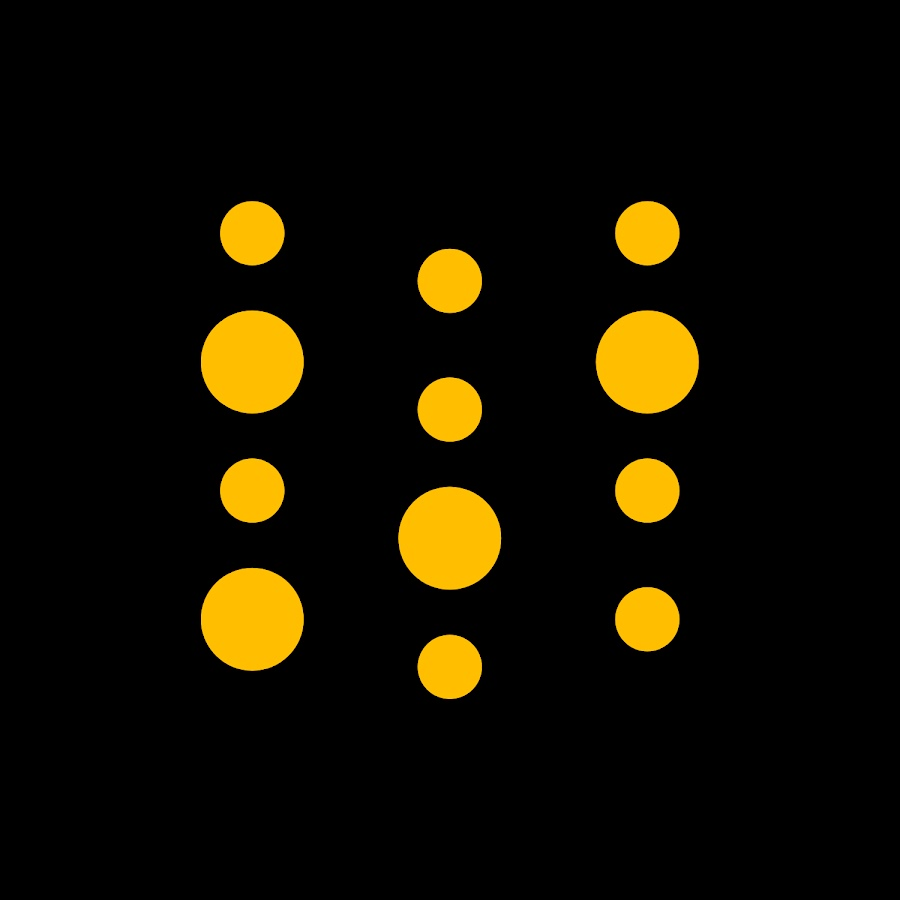
\includegraphics[width = 2cm]{images/wandb.png}} &
      \subfloat[TensorBoard]{
\includegraphics[width = 2cm]{images/tensorboard.png}} &
      \subfloat[Neptune]{
\includegraphics[width = 2cm]{images/neptune.png}} \\
      \subfloat[Guild AI]{
\includegraphics[width = 2cm]{images/guildai.jpg}} &
      \subfloat[Comet]{
\includegraphics[width = 2cm]{images/coemt.png}}
      \end{tabular}
      \caption{Machine Learning Data Visualization Tools}
    \end{figure}
  \end{frame}

  \section{Analysis}
  \begin{frame}{Domain}
    \begin{figure}
      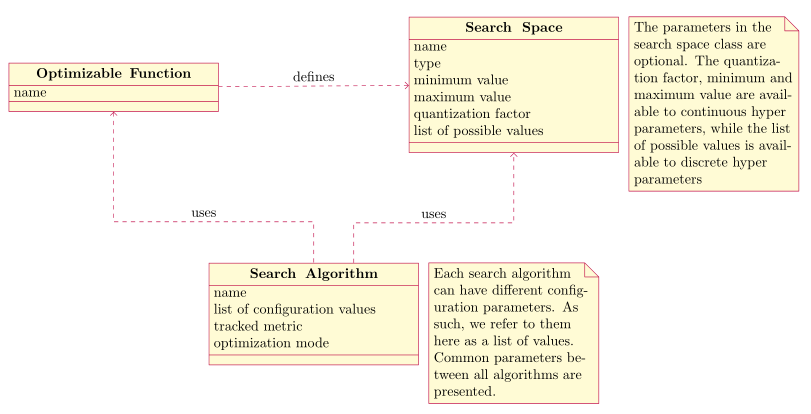
\includegraphics[width=\textwidth]{images/domain_model.png}
      \caption{Domain Model}
    \end{figure}
  \end{frame}
  \begin{frame}{Requirements}
    The requirements for this project was using the FURPS+ model.
  \end{frame}
  \begin{frame}{Functionality}
    \begin{itemize}
      \item A privileged developer can integrate new HPO algorithms into the framework
      \item A developer can define all necessary information to allow the optimization pipeline to run (hyper parameter definitions, objective function instantiation, algorithm selection, etc.)
      \item A developer can obtain information during and at the end of the optimization process regarding said process
      \item A developer can run the optimization pipeline.
    \end{itemize}
  \end{frame}
  \begin{frame}{Usability}
    \begin{itemize}
      \item There should be comprehensive documentation on how the system functions and how a user interacts with it
      \item There should be pre-existing examples of usage of the system.
    \end{itemize}
  \end{frame}
  \begin{frame}{Reliability}
    \begin{itemize}
      \item The system should be able to recover from external failures (eg.\ issues with CAM2\textsuperscript{\textregistered})
      \item The system should be able to save its state in order to allow for interruptions in the execution.
    \end{itemize}
  \end{frame}
  \begin{frame}{Performance}
    \begin{itemize}
      \item The software should be faster than the CAM2\textsuperscript{\textregistered}'s endpoints it accesses
      \item The software should be efficient in such a way that it does not interfere with the CAM2\textsuperscript{\textregistered} software
      \item The system should consume as little resources as possible, allowing for it to be run directly in the developer's issued laptop, without interfering with other programs.
    \end{itemize}
  \end{frame}
  \begin{frame}{Supportability}
    \begin{itemize}
      \item The developed code should include meaningful testing, insuring the correct operation of the software
      \item The developed system should allow for extending its usage to new algorithms and optimizable functions
      \item The developer should be able to define their preferred configuration when executing the software
      \item The software should be installable in any of \farons's issued laptop easily.
    \end{itemize}
  \end{frame}
  \begin{frame}{Design Constraints}
    \begin{itemize}
      \item The developed application must be implemented in Python.
    \end{itemize}
  \end{frame}
  \begin{frame}{Implementation Constraints}
    \begin{itemize}
      \item The developed application must executed with minimal resource allocation (with regards to CPU usage and RAM allocation)
      \item The developed application must be able to execute in a Windows environment.
    \end{itemize}
  \end{frame}
  \begin{frame}{Interface Constraints}
    \begin{itemize}
      \item The optimization pipeline must allow communication with the CAM2\textsuperscript{\textregistered} integrated web server
      \item Said communication must be executed through HTTP, using pre existing endpoints.
    \end{itemize}
  \end{frame}
  \begin{frame}{Physical Constraints}
    \begin{itemize}
      \item The developed system should be executed in the same network as the CAM2\textsuperscript{\textregistered} integrated web server.
    \end{itemize}
  \end{frame}

  \section{Design}
  \begin{frame}{Context}
    hello world
  \end{frame}
  \begin{frame}{Containers}
    hello world
  \end{frame}
  \begin{frame}{Components}
    hello world
  \end{frame}
  \begin{frame}{Code}
    hello world
  \end{frame}

  \section{Implementation}
  \begin{frame}{Description}
    hello world
  \end{frame}
  \begin{frame}{Tests}
    hello world
  \end{frame}
  \begin{frame}{Evaluation}
    DEMO HERE
  \end{frame}

  \section{Conclusion}
  \begin{frame}{Objectives}
    hello world
  \end{frame}
  \begin{frame}{Limitations and Future Work}
    hello world
  \end{frame}
  \begin{frame}{Final Remarks}
    hello world
  \end{frame}


\end{document}
